\documentclass[11pt]{../../TexTemplate/elegantbook} % 这里是文档类,默认使用 elegantbook

\title{Géométrie Analytique} % 这里放置书名
% \subtitle{Subtitle} % 这里放置副标题

\author{CatMono} % 这里放置作者名
\date{October, 2025} % 这里放置日期
\version{0.1} % 这里放置版本号
% \institute{Elegant\LaTeX{} Program} % 这里放置机构名
% \bioinfo{Custom Key}{Custom Value} % 这里放置自定义信息

% \extrainfo{extra information} % 这里放置额外信息,将显示在最下方中央

\setcounter{tocdepth}{2} % 设置目录深度
\setcounter{secnumdepth}{2} % 设置章节编号深度


% \logo{logo-blue.png} % 这里放置封面logo,默认从figure目录下寻找
% \cover{LogiqueMathematique.png} % 这里放置封面图片,默认从figure目录下寻找

% modify the color in the middle of titlepage
\definecolor{customcolor}{RGB}{32,178,170} % 自定义颜色
\colorlet{coverlinecolor}{customcolor}
\usepackage{cprotect} % 保护命令参数不被 LaTeX 解析器过早处理,允许在某些特殊环境中使用脆弱命令(fragile commands)。
\usepackage{xeCJK} % 使用 xeCJK 包支持中文
\usepackage{extarrows} % 使用 extarrows 包支持数学公式


% ===== 开始文档 =====
\begin{document}

\maketitle %生成文档的标题页,根据之前定义的标题信息(如标题、作者、日期等)自动创建一个格式化的标题页

% === 前言部分 ===
\frontmatter        % 开始前言,页码为 i, ii, iii...
\tableofcontents    % 目录 (页码: i, ii)
% \listoffigures      % 图表目录 (页码: iii)
% \listoftables       % 表格目录 (页码: iv)

\chapter{Preface}   % 前言章节(无编号,页码: v, vi...)
Without other remarks, this book is based on the \(\mathbb{R}^{3}\) space.

% \chapter{Acknowledgments}  % 致谢(无编号)
% I would like to thank...
% === 正文部分 ===
\mainmatter         % 开始正文,页码从 1 重新开始

\chapter{Preliminaries} % 这里放置章节标题

\chapter{Coordinates and Vectors}
\section{Coordinate Systems}
\begin{definition}{Coordinate Frame}
    A fixed point \(O\) in \(\mathbb{R}^{3}\) space,
    together with three non-coplanar ordered vectors \(\mathbf{e}_{1}, \mathbf{e}_{2}, \mathbf{e}_{3}\),
    is called a \textbf{coordinate frame} (or \textbf{reference frame}) in space,
    denoted by \(\{O ; \mathbf{e}_{1}, \mathbf{e}_{2}, \mathbf{e}_{3}\}\).

    If \(\mathbf{e}_{1}, \mathbf{e}_{2}, \mathbf{e}_{3}\) are unit vectors,
    then the frame is called a \textbf{Cartesian frame}.
    Furthermore, if \(\mathbf{e}_{1} \perp \mathbf{e}_{2}, \mathbf{e}_{2} \perp \mathbf{e}_{3}, \mathbf{e}_{3} \perp \mathbf{e}_{1}\),
    then the frame is called a \textbf{rectangular Cartesian frame}, or simply a \textbf{rectangular frame}.

    Generally, \(\{O ; \mathbf{e}_{1}, \mathbf{e}_{2}, \mathbf{e}_{3}\}\) is called \textbf{affine frame}.
\end{definition}

\section{Theorems about Vectors}

\section{Products of Vectors}
\begin{leftbarTitle}{Inner Product (Dot Product)}\end{leftbarTitle}

\begin{leftbarTitle}{Outer Product (Cross Product)}\end{leftbarTitle}

\begin{leftbarTitle}{Mixed Product}\end{leftbarTitle}

\begin{leftbarTitle}{Double Cross Product}\end{leftbarTitle}

\section{Linear Independence}

\chapter{Locus and Equation}
\section{Parametric Equations}

\section{Common Curves and Surfaces}

\chapter{Planes and Space Lines}
\section{Equations of Planes}
\begin{leftbarTitle}{Point-Vector Form}\end{leftbarTitle}
In space, fix a point \(M_{0} = (X_{0}, Y_{0}, Z_{0})\) and two non-collinear vectors \(\mathbf{a} = (X_{1}, Y_{1}, Z_{1})\) 
and \(\mathbf{b} = (X_{2}, Y_{2}, Z_{2})\).
The equation of the plane passing through the point \(M_{0}\) and 
parallel to the vectors \(\mathbf{a}\) and \(\mathbf{b}\) is given by:
\[
\mathbf{r} = \vec{OM} + \lambda \mathbf{a} + \mu \mathbf{b},
\]
or in coordinate form:
\[
\begin{cases}
x = X_{0} + \lambda X_{1} + \mu X_{2} \\
y = Y_{0} + \lambda Y_{1} + \mu Y_{2} \\
z = Z_{0} + \lambda Z_{1} + \mu Z_{2}
\end{cases}
\]
where \(\lambda, \mu \in \mathbb{R}\).

Taking the dot product of both sides of the parametric vector equation with \(\mathbf{a} \times \mathbf{b}\), 
we eliminate \(\lambda\) and \(\mu\) to obtain \((\mathbf{r} - \vec{OM_{0}}, \mathbf{a}, \mathbf{b}) = 0\), that is,
\begin{equation}\label{eq:PlaneDeterminantForm}
    \begin{vmatrix}
        x - X_{0} & y - Y_{0} & z - Z_{0} \\
        X_{1} & Y_{1} & Z_{1} \\
        X_{2} & Y_{2} & Z_{2}
    \end{vmatrix} = 0.
\end{equation}
All above forms are called the \textbf{point-vector form} of the plane equation.
\vspace{0.7cm}

Given three non-collinear points \(M_{1}(X_{1}, Y_{1}, Z_{1})\), \(M_{2}(X_{2}, Y_{2}, Z_{2})\) and \(M_{3}(X_{3}, Y_{3}, Z_{3})\),
the equation of the plane passing through these three points is given by:
\[
\mathbf{r} = \vec{OM_{1}} + \lambda \vec{M_{1}M_{2}} + \mu \vec{M_{1}M_{3}},
\]
or in coordinate form:
\[
\begin{cases}
x = X_{1} + \lambda (X_{2} - X_{1}) + \mu (X_{3} - X_{1}) \\
y = Y_{1} + \lambda (Y_{2} - Y_{1}) + \mu (Y_{3} - Y_{1}) \\
z = Z_{1} + \lambda (Z_{2} - Z_{1}) + \mu (Z_{3} - Z_{1})
\end{cases}
\]
where \(\lambda, \mu \in \mathbb{R}\).
And the determinant form is:
\[
\begin{vmatrix}
x - X_{1} & y - Y_{1} & z - Z_{1} \\
X_{2} - X_{1} & Y_{2} - Y_{1} & Z_{2} - Z_{1} \\
X_{3} - X_{1} & Y_{3} - Y_{1} & Z_{3} - Z_{1}
\end{vmatrix} = 0,
\]
or equivalently,
\[
\begin{vmatrix}
x & y & z & 1 \\
X_{1} & Y_{1} & Z_{1} & 1 \\
X_{2} & Y_{2} & Z_{2} & 1 \\
X_{3} & Y_{3} & Z_{3} & 1
\end{vmatrix} = 0.
\]
All above forms are also called the \textbf{three-point form} of the plane equation.

If plane intersects the three coordinate axes at 
\(M_{1}(X_{1}, 0, 0)\), \(M_{2}(0, Y_{2}, 0)\), \(M_{3}(0, 0, Z_{3})\) (where \(X_{1}, Y_{2}, Z_{3} \neq 0\)), 
then the equation of the plane can be expressed in the form:
\[
\frac{x}{X_{1}} + \frac{y}{Y_{2}} + \frac{z}{Z_{3}} = 1,
\]
which is called the \textbf{intercept form} of the plane equation.

\begin{leftbarTitle}{General Form}\end{leftbarTitle}
The general equation is obtained by expanding the determinant form of 
the parametric equation~\ref{eq:PlaneDeterminantForm} of a plane:
\[
Ax + By + Cz + D = 0,
\]
where
\[
A = \begin{vmatrix} Y_{1} & Z_{1} \\ Y_{2} & Z_{2} \end{vmatrix}, \quad
B = \begin{vmatrix} Z_{1} & X_{1} \\ Z_{2} & X_{2} \end{vmatrix}, \quad
C = \begin{vmatrix} X_{1} & Y_{1} \\ X_{2} & Y_{2} \end{vmatrix}, \quad
D = -\begin{vmatrix} X_{0} & Y_{0} & Z_{0} \\ X_{1} & Y_{1} & Z_{1} \\ X_{2} & Y_{2} & Z_{2} \end{vmatrix}.
\]
Special cases include:

\begin{theorem}
    Any plane in space can be represented by a linear equation in three variables \(x\), \(y\), and \(z\), 
    and conversely, every such equation represents a plane in space.
\end{theorem}

\begin{leftbarTitle}{Point-Normal Form}\end{leftbarTitle}
Given a point \(M_{0}(X_{0}, Y_{0}, Z_{0})\) on the plane and a normal vector \(\mathbf{n} = (A, B, C)\) of the plane,
the equation of the plane can be expressed as:
\[
\mathbf{n} \cdot (\mathbf{r} - \vec{OM_{0}}) = 0,
\]
or in coordinate form:
\[
A(x - X_{0}) + B(y - Y_{0}) + C(z - Z_{0}) = 0.
\]
If a perpendicular is drawn from the origin to the plane, 
with the foot of the perpendicular being \(M_{0}(X_{0}, Y_{0}, Z_{0})\), 
and the unit normal vector of the plane being \(\mathbf{n_{0}} = (\cos \alpha, \cos \beta, \cos \gamma)\), then
\[
\mathbf{n} \cdot \mathbf{r} - \vec{OM_{0}} = 0,
\]
or in coordinate form:
\begin{equation}\label{eq:PlanePointNormalUnitForm}
    x \cos \alpha + y \cos \beta + z \cos \gamma - |\vec{OM_{0}}| = 0.    
\end{equation}

For the general equation of a plane, 
it can be converted into the form~\ref{eq:PlanePointNormalUnitForm} 
by simply multiplying by a \textbf{normalization factor} \(\lambda\), where:
\[
|\lambda| = \frac{1}{|\mathbf{n}|} = \frac{1}{\sqrt{A^2 + B^2 + C^2}},
\]
and \(\lambda\) has the opposite sign as \(D\).

\section{Linear Equations}
\begin{leftbarTitle}{Point-Vector Form}\end{leftbarTitle}
Given a point \(M_{0}(X_{0}, Y_{0}, Z_{0})\) in space and a direction vector \(\mathbf{v} = (X, Y, Z)\) of the line, 
then
\[
\mathbf{r} = \vec{OM_{0}} + \lambda \mathbf{v},
\]
and the parametric equations of the line can be expressed as:
\[
\begin{cases}
x = X_{0} + \lambda X \\
y = Y_{0} + \lambda Y \\
z = Z_{0} + \lambda Z
\end{cases}
\]
where \(\lambda \in \mathbb{R}\).
Eliminate the parameter \(\lambda\) to obtain the symmetric equation (standard equation):
\begin{equation}\label{eq:LineSymmetricForm}
    \frac{x - X_{0}}{X} = \frac{y - Y_{0}}{Y} = \frac{z - Z_{0}}{Z}.
\end{equation}

\vspace{0.7cm}
Given two points \(M_{1}(X_{1}, Y_{1}, Z_{1})\) and \(M_{2}(X_{2}, Y_{2}, Z_{2})\) in space,
the equation of the line passing through these two points is given by:
\[
\mathbf{r} = \vec{OM_{1}} + \lambda \vec{M_{1}M_{2}},
\]
or in coordinate form:
\[
\begin{cases}
x = X_{1} + \lambda (X_{2} - X_{1}) \\
y = Y_{1} + \lambda (Y_{2} - Y_{1}) \\
z = Z_{1} + \lambda (Z_{2} - Z_{1}).
\end{cases}
\]
It can also be expressed in symmetric form:
\[
\frac{x - X_{1}}{X_{2} - X_{1}} = \frac{y - Y_{1}}{Y_{2} - Y_{1}} = \frac{z - Z_{1}}{Z_{2} - Z_{1}}.
\]

The coordinates of the direction vector of a line, \(X, Y, Z\), or a set of numbers proportional to it, 
\(l, m, n\) \((l : m : n = X : Y : Z)\), are called the \textbf{direction numbers} of the line.

\begin{leftbarTitle}{General Form}\end{leftbarTitle}
The intersection of two planes determines a line:
\[
\begin{cases}
A_{1}x + B_{1}y + C_{1}z + D_{1} = 0 \\
A_{2}x + B_{2}y + C_{2}z + D_{2} = 0,
\end{cases}
\]
where \(A_{1} : B_{1} : C_{1} \neq A_{2} : B_{2} : C_{2}\)

\begin{theorem}
    Any line in space can be represented by a system of two linear equations in three variables \(x\), \(y\), and \(z\),
    and conversely, every such system represents a line in space.
    
\end{theorem}

\begin{leftbarTitle}{Projection Form}\end{leftbarTitle}
In the symmetric equation~\ref{eq:LineSymmetricForm} of a line,
\(X\), \(Y\), and \(Z\) are not all zero. 
Without loss of generality, let us assume \(Z\) is not zero. 
Then, we have:
\[
\begin{cases}
    x = az + c \\
    y = bz + d,
\end{cases}
\]
where \(a = \frac{X}{Z}\), \(b = \frac{Y}{Z}\), \(c = X_{0} - \frac{X}{Z}Z_{0}\), and \(d = Y_{0} - \frac{Y}{Z}Z_{0}\).
This form is called the \textbf{projection form} of the line equation.
This line can be regarded as the intersection line of the two planes represented by these two equations. 
These planes are respectively parallel to the \(y\)-axis and \(x\)-axis, 
and perpendicular to the \(xOz\) and \(yOz\) coordinate planes.


\section{Relative Positions of Points, Lines and Planes}
\begin{leftbarTitle}{Points and Lines}\end{leftbarTitle}
There are only two possible relative positions between a point and a line:
the point is either on the line or it is not.
This can be determined by simply checking if the coordinates of the point satisfy the line's equation.

When the point \(M_{0}(X_{0}, Y_{0}, Z_{0})\) is not on the line
\[
l: \frac{x - X_{1}}{X} = \frac{y - Y_{1}}{Y} = \frac{z - Z_{1}}{Z},
\]
the distance from the point to the line is given by:
\[
d = \frac{|(\vec{M_{1}M_{0}}, \mathbf{v})|}{|\mathbf{v}|},
\]
where \(\vec{M_{1}M_{0}} = (X_{0} - X_{1}, Y_{0} - Y_{1}, Z_{0} - Z_{1})\),
\(M_{1}(X_{1}, Y_{1}, Z_{1})\) is a point on the line,
\(\mathbf{v}\) is the direction vector of the line.



\begin{leftbarTitle}{Points and Planes}\end{leftbarTitle}
The relative position between a point and a plane 
can be determined by checking if the coordinates of the point satisfy the plane's equation.
The distance is given below.

\begin{definition}{Deviation}
    From point \(M_{0} = (X_{0}, Y_{0}, Z_{0})\), 
    a perpendicular is drawn to the plane \(A x + B y + C z + D = 0\) with the foot of the perpendicular being \(Q\)
    ~(Fig \ref{fig:DeviationOfPointFromPlane}). 
    The projection of the vector \(\vec{QM_{0}}\) onto the unit normal vector \(\mathbf{n}_{0}\) of the plane 
    is called the \textbf{deviation} of point \(M_{0}\) from the plane, 
    denoted as: 
    \[
    \delta = \mathrm{Pr}_{\mathbf{n}_{0}} \vec{QM_{0}}.
    \]
\end{definition}
\begin{figure}[h]
    \centering
    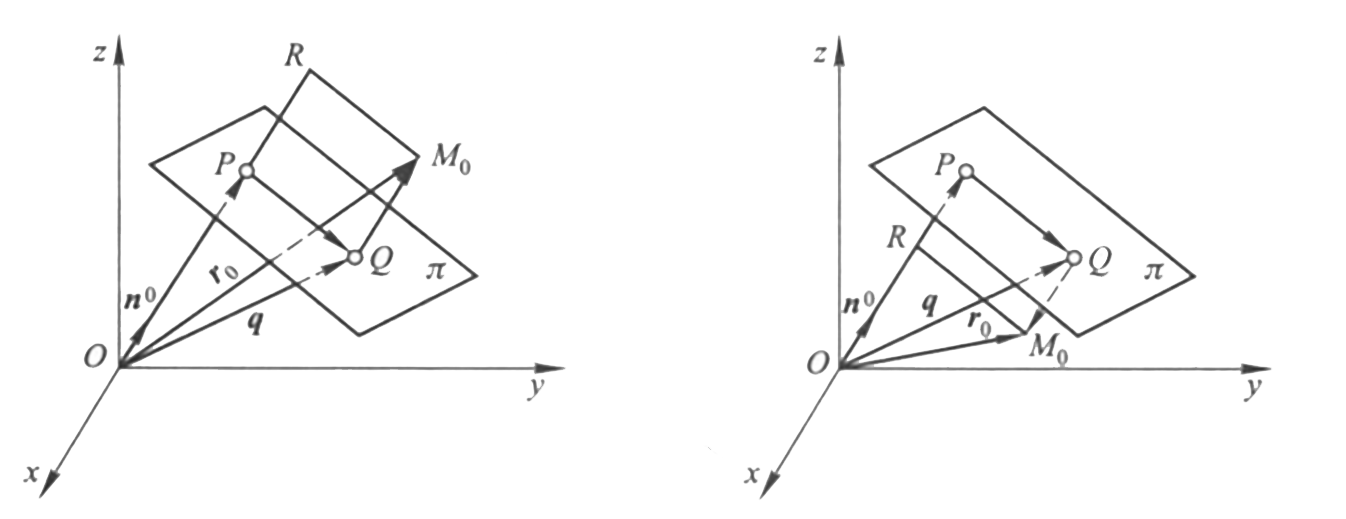
\includegraphics[width=0.8\textwidth]{img/deviation.png}
    \caption{Deviation of a Point from a Plane.}
    \label{fig:DeviationOfPointFromPlane}
\end{figure}

Obviously, the absolute value of the deviation is equal to the distance from the point to the plane.
The deviation can be calculated using the formula:
\begin{align*}
    \delta &= \mathbf{n}_{0} \cdot \vec{OM_{0}} - |\vec{OP}|\\ 
    &= X_{0}\cos \alpha + Y_{0}\cos \beta + Z_{0}\cos \gamma - |\vec{OP}| \\
    &= \lambda (A X_{0} + B Y_{0} + C Z_{0} + D) \\
    &= \pm \frac{A X_{0} + B Y_{0} + C Z_{0} + D}{\sqrt{A^2 + B^2 + C^2}}.
\end{align*}
For points on the same side of a plane, the deviation signs are the same; 
for points on opposite sides, the signs are different; 
if the deviation is \(0\), the point lies on the plane.


\begin{leftbarTitle}{Lines and Lines}\end{leftbarTitle}
For two lines in space
\begin{gather*}
    l_{1}: \frac{x - x_{1}}{X_{1}} = \frac{y - y_{1}}{Y_{1}} = \frac{z - z_{1}}{Z_{1}}, \\
    l_{2}: \frac{x - x_{2}}{X_{2}} = \frac{y - y_{2}}{Y_{2}} = \frac{z - z_{2}}{Z_{2}}.
\end{gather*}
Relative positions can be classified into four cases:
\begin{description}
    \item[Skew] 
    \[\Delta = \begin{vmatrix}
        x_{2} - x_{1} & y_{2} - y_{1} & z_{2} - z_{1} \\
        X_{1} & Y_{1} & Z_{1} \\
        X_{2} & Y_{2} & Z_{2} \\
    \end{vmatrix} \neq 0
    \]
    \item[Intersecting] \(\Delta = 0, X_{1}:Y_{1}:Z_{1}\neq X_{2}:Y_{2}:Z_{2}\)
    \item[Parallel] \(X_{1}:Y_{1}:Z_{1} = X_{2}:Y_{2}:Z_{2} \neq (x_{2}-x_{1}): (y_{2}-y_{1}): (z_{2}-z_{1})\)
    \item[Coincident] \(X_{1}:Y_{1}:Z_{1} = X_{2}:Y_{2}:Z_{2} = (x_{2}-x_{1}): (y_{2}-y_{1}): (z_{2}-z_{1})\)
\end{description}

\begin{definition}{Common Perpendicular}
    The line that is perpendicular and intersects two skew lines is called 
    the \textbf{common perpendicular} of the two skew lines, 
    and the length of the segment between the two points of intersection is called the length of the common perpendicular.    
\end{definition}
\begin{figure}[h]
    \centering
    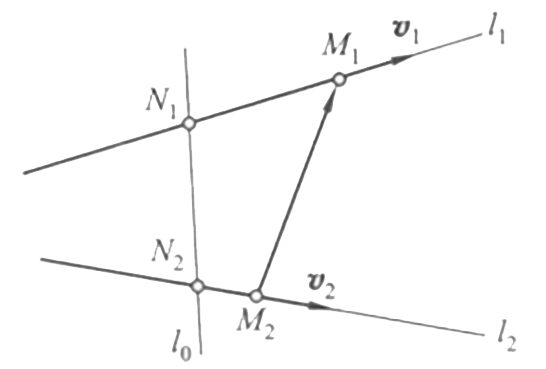
\includegraphics[width=0.6\textwidth]{img/CommonPerp.png}
    \caption{Common Perpendicular of Two Skew Lines.}
    \label{fig:CommonPerpendicular}
\end{figure}
The length of the common perpendicular between two skew lines is given by:
\[
d = \frac{|(\vec{M_{1}M_{2}}, \mathbf{v_{1}}, \mathbf{v_{2}})|}{|\mathbf{v_{1}} \times \mathbf{v_{2}}|}.
\]
The common perpendicular can be seen as the intersection of two planes:
\begin{gather*}
    \pi_{1}: (\mathbf{r} - \vec{OM_{1}}, \mathbf{v}_{1}, \mathbf{v}_{1}\times \mathbf{v}_{2}) = 0, \\
    \pi_{2}: (\mathbf{r} - \vec{OM_{2}}, \mathbf{v}_{2}, \mathbf{v}_{1}\times \mathbf{v}_{2}) = 0.
\end{gather*}
Since the equation of the common perpendicular is:
\[
\begin{cases} \det\begin{pmatrix}x-x_{1}&y-y_{1}&z-z_{1}\\X_{1}&Y_{1}&Z_{1}\\X&Y&Z\end{pmatrix}=0,  \\ 
    \det\begin{pmatrix}x-x_{2}&y-y_{2}&z-z_{2}\\X_{2}&Y_{2}&Z_{2}\\X&Y&Z\end{pmatrix}=0,
\end{cases}
\]
where \((X, Y, Z) = \mathbf{v_{1}} \times \mathbf{v_{2}}\).

\begin{property}
    \begin{itemize}
        \item The common perpendicular to two skew lines exists and is unique.
        \item The length of the common perpendicular segment between two skew lines is the distance between them.
    \end{itemize}
\end{property}


\begin{leftbarTitle}{Lines and Planes}\end{leftbarTitle}

\begin{leftbarTitle}{Planes and Planes}\end{leftbarTitle}


\section{Pencil of Planes and Lines}

\chapter{Common Surfaces}
\section{Cylinder Surfaces}
\begin{definition}{Cylinder Surface}
    In space, the surface generated by a family of parallel lines, 
    which are parallel to a fixed direction (the direction of the cylinder \[\mathbf{s} = (X : Y : Z)\]) 
    and intersect a fixed curve (the directrix \[\Gamma : \mathbf{\begin{cases} F_{1}(x,y,z) = 0,\\ F_{2}(x,y,z) = 0,\end{cases}}\]), 
    is called a \textbf{cylinder}.
\end{definition}
Cylinder can be expressed as:
\begin{align*}
    &\{ (x,y,z) | F(x,y,z) = 0 \} \\
    =&\bigcup_{(x_{1},y_{1},z_{1}) \in \Gamma} \{ (x,y,z) | \frac{x - x_{1}}{X} = \frac{y - y_{1}}{Y} = \frac{z - z_{1}}{Z} \}\\
    \xlongequal{\text{directrix } \Gamma:\mathbf{r}(u)=(x(u),y(u),z(u))}
    &\{ \mathbf{r} | \mathbf{r} = \mathbf{r}(u)+v \mathbf{s},\quad u,v \in \mathbb{R} \} \\
    \xlongequal{\text{parametric form}}
    &  \left\{ (x,y,z) | \begin{cases} x = x(u) + vX, \\ y = y(u) + vY, \\ z = z(u) + vZ, \end{cases}\quad u,v \in \mathbb{R} \right\}.
\end{align*}
To solve the equation of a cylinder,
\[
\begin{cases}
    \frac{x - x_{1}}{X} = \frac{y - y_{1}}{Y} = \frac{z - z_{1}}{Z}, \\
    F_{1}(x_{1},y_{1},z_{1}) = 0, \\
    F_{2}(x_{1},y_{1},z_{1}) = 0.
\end{cases}
\]

\vspace{0.7cm}
Some special cases of cylinders (in~\ref{fig:CylinderSurface}):
\begin{description}
    \item[Elliptical Cylinder] \(\frac{x^2}{a^2} + \frac{y^2}{b^2} = 1\)
    \item[Hyperbolic Cylinder] \(\frac{x^2}{a^2} - \frac{y^2}{b^2} = 1\)
    \item[Parabolic Cylinder] \(y^{2} = 2px\)
\end{description}
Their equations are all quadratic, so they are collectively called \textbf{quadratic cylinders}.

\begin{figure}[h]
    \centering
    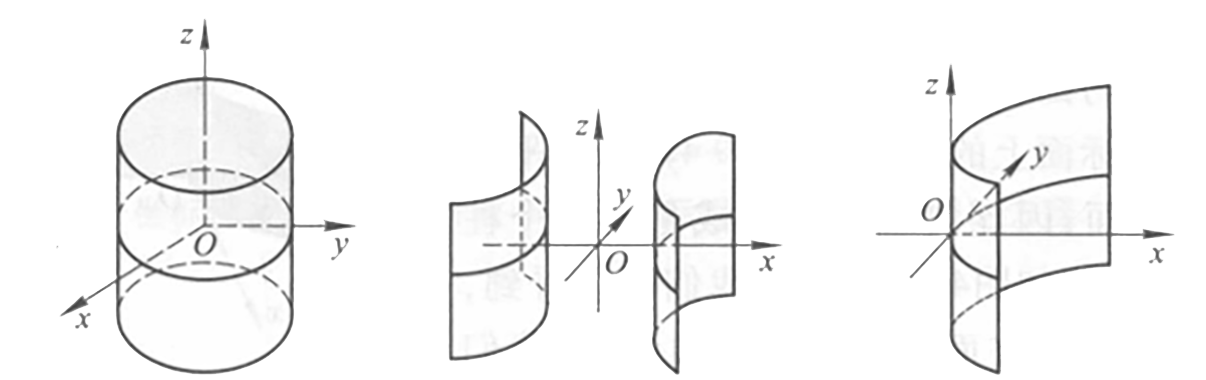
\includegraphics[width=0.8\textwidth]{img/Cylinder.png}
    \caption{Cylinder Surface.}
    \label{fig:CylinderSurface}
\end{figure}

When a plane intersects a elliptical cylinder to form an ellipse (or a circle), the following rules apply:
\begin{enumerate}
    \item  The center of the resulting ellipse lies on the axis of the cylindrical surface.
    \item  \(b = R\), meaning the length of the semi-minor axis of the ellipse is equal to the radius of the cylindrical surface.
    \item  \(\sin \theta = \frac{R}{a}\), where \(a\) represents the length of the semi-major axis of the ellipse, 
        and \(\theta\) represents the angle between the axis of the cylinder and the plane.
\end{enumerate}


\vspace{0.7cm}
\begin{theorem}
    In a spatial Cartesian coordinate system (as well as in an affine coordinate system), 
    a surface represented by a ternary equation containing only two variables (coordinates) 
    is a cylinder whose generatrices are parallel to the coordinate axis corresponding to the missing variable (coordinate).
\end{theorem}

\begin{example}
    
\end{example}

\begin{note}
    Two methods to prove that an equation is a cylindrical surface: 
    \begin{enumerate}
        \item Rewrite as a product equation using determinants and linear systems.
        \item Take the directrix, set the direction, solve, and compare.
    \end{enumerate}
\end{note}

\section{Cone Surfaces}
\begin{definition}{Cone Surface}
    In space, the surface generated by a family of lines passing through a fixed point 
    (the vertex \[A:\mathbf{r}_{0}=(x_{0},y_{0},z_{0})\]) 
    and intersecting a fixed curve 
    (the directrix \[\Gamma : \mathbf{\begin{cases} F_{1}(x,y,z) = 0,\\ F_{2}(x,y,z) = 0,\end{cases}}\]), 
    is called a \textbf{cone}.
\end{definition}
Cone can be expressed as:
\begin{align*}
    &\{ (x,y,z) | F(x,y,z) = 0 \} \\
    =&\bigcup_{(x_{1},y_{1},z_{1}) \in \Gamma} \{ (x,y,z) | \frac{x - x_{0}}{x_{1} - x_{0}} = \frac{y - y_{0}}{y_{1} - y_{0}} = \frac{z - z_{0}}{z_{1} - z_{0}} \}\\
    \xlongequal{\text{directrix } \Gamma:\mathbf{r}(u)=(x(u),y(u),z(u))}
    &\{ \mathbf{r} | \mathbf{r} = \mathbf{r}_{0}+v (\mathbf{r}(u)-\mathbf{r}_{0}),\quad u,v \in \mathbb{R} \} \\
    \xlongequal{\text{parametric form}}
    &  \left\{ (x,y,z) | \begin{cases} x = x_{0} + v(x(u) - x_{0}), \\ y = y_{0} + v(y(u) - y_{0}), \\ z = z_{0} + v(z(u) - z_{0}), \end{cases}\quad u,v \in \mathbb{R} \right\}.
\end{align*}
To solve the equation of a cone,
\[
\begin{cases}
    \frac{x - x_{0}}{x_{1} - x_{0}} = \frac{y - y_{0}}{y_{1} - y_{0}} = \frac{z - z_{0}}{z_{1} - z_{0}}, \\
    F_{1}(x_{0},y_{0},z_{0}) = 0, \\
    F_{2}(x_{0},y_{0},z_{0}) = 0.
\end{cases}
\]

\vspace{0.7cm}
\begin{theorem}
    A homogeneous equation in \(x, y, z\) always represents a cone with its vertex at the origin.
    That is, a homogeneous equation in \(x-x_{0}, y-y_{0}, z-z_{0}\) always represents a cone 
    with its vertex at \((x_{0}, y_{0}, z_{0})\).
\end{theorem}


\section{Surfaces of Revolution}
\begin{definition}{Surface of Revolution}
    In space, the surface generated by rotating a curve 
    (the generatrix \[\Gamma : \begin{cases} F_{1}(x,y,z)=0, \\ F_{2}(x,y,z)=0, \end{cases}\]) 
    around a fixed straight line 
    (the axis of revolution \[l: \frac{x-x_{0}}{X} = \frac{y-y_{0}}{Y} = \frac{z-z_{0}}{Z}\]) 
    is called a \textbf{surface of revolution}.

    Any point \(M_{1}(x_{1},y_{1},z_{1})\) on the generatrix \(\Gamma\) of a surface of revolution 
    generates a circle upon rotation, which is called a \textbf{parallel}; 
    the intersection of the surface with each half-plane bounded by \(l\) is called a \textbf{meridian}.
\end{definition}
Surface of revolution can be expressed as:
\begin{align*}
    &\{ (x,y,z) | F(x,y,z) = 0 \} \\
    =&\bigcup_{(x_{1},y_{1},z_{1}) \in \Gamma} 
    \left\{ (x,y,z) | \begin{cases} X(x-x_{1})+Y(y-y_{1})+Z(z-z_{1}) = 0, \\ 
        (x-x_{0})^{2} + (y-y_{0})^{2} + (z-z_{0})^{2} = (x-x_{1})^{2} + (y-y_{1})^{2} + (z-z_{1})^{2} \end{cases} \right\} \\
\end{align*}

Taking the plane of the directrix as the coordinate plane and the axis of rotation as the coordinate axis, 
the equation of the surface of revolution assumes a special form (see~\ref{fig:SurfaceOfRevolution}).
\begin{figure}[h]
    \centering
    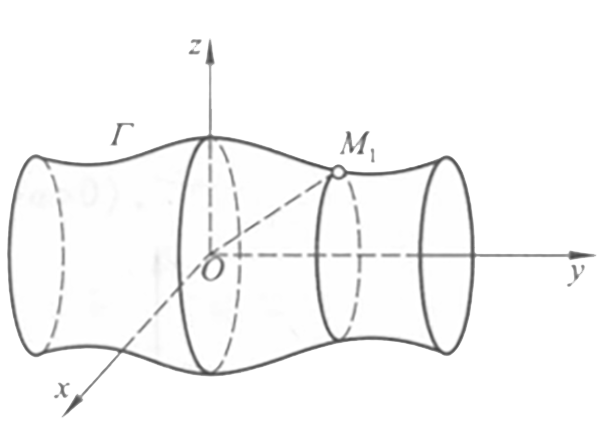
\includegraphics[width=0.4\textwidth]{img/Revolution.png}
    \caption{Surface of Revolution.}
    \label{fig:SurfaceOfRevolution}
\end{figure}
As shown in the figure, the generatrix is
\[
\Gamma: \begin{cases} F(y,z)=0, \\ x = 0. \end{cases}
\]
The equation obtained by rotating around the \(y\)-axis is
\[
F(y, \pm \sqrt{x^{2}+z^{2}}) = 0.
\]
Similarly, the equation obtained by rotating around the \(z\)-axis is 
\[
F(\pm \sqrt{x^{2}+y^{2}}, z) = 0.
\]
That is: retain the coordinate that shares the name with the axis of rotation, 
and express the other coordinate in the equation as the square root of the sum of the squares of the other two coordinates. 
Based on this pattern of the equation for a surface of revolution, 
it is also possible to determine in reverse whether an equation represents a surface of revolution.

\vspace{0.7cm}
Some special cases of surfaces of revolution:

\noindent Rotate ellipse
\[
\Gamma: \begin{cases} \frac{x^{2}}{a^{2}} + \frac{y^{2}}{b^{2}} = 1,\quad(a>b) \\ z = 0, \end{cases}
\]
\begin{itemize}
    \item around \(x\)-axis (long axis): \( \frac{x^{2}}{a^{2}} + \frac{y^{2}}{b^{2}} + \frac{z^{2}}{b^{2}} = 1\) (prolate spheroid) 
    \item around \(y\)-axis (short axis): \( \frac{x^{2}}{a^{2}} + \frac{y^{2}}{b^{2}} + \frac{z^{2}}{a^{2}} = 1\) (oblate spheroid)
\end{itemize}
(see~\ref{fig:Ellipsoids}).
\begin{figure}[h]
    \centering
    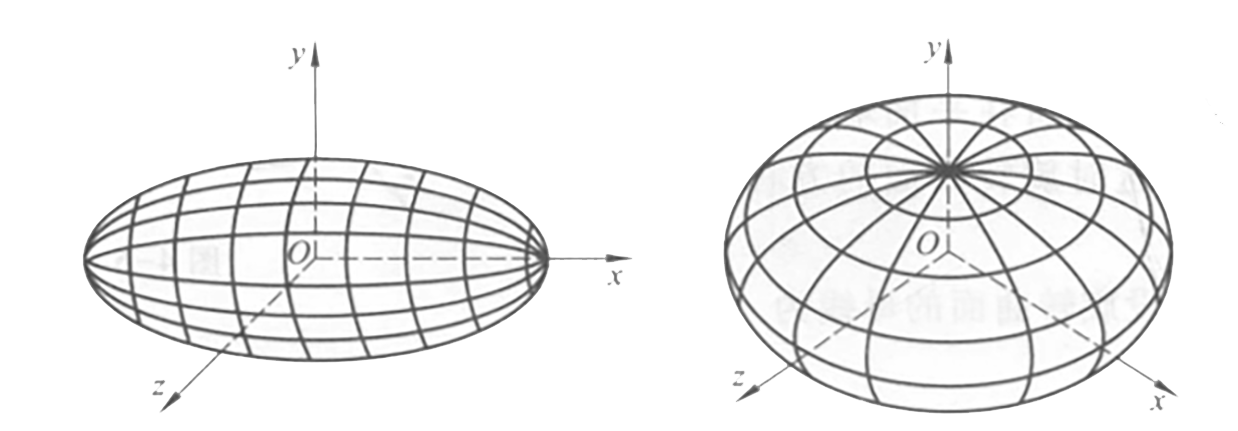
\includegraphics[width=0.6\textwidth]{img/ellipse.png}
    \caption{Ellipsoids.}
    \label{fig:Ellipsoids}
\end{figure}

\noindent Rotate hyperbola
\[
\Gamma: \begin{cases} \frac{y^{2}}{b^{2}}-\frac{z^{2}}{c^{2}} = 1,\quad (b>c) \\ x = 0, \end{cases}
\]
\begin{itemize}
    \item around \(y\)-axis (real axis): \( \frac{y^{2}}{b^{2}} - \frac{x^{2}}{c^{2}} - \frac{z^{2}}{b^{2}} = 1\) 
        (two-sheet hyperboloid) 
    \item around \(z\)-axis (unreal axis): \( \frac{x^{2}}{b^{2}} + \frac{y^{2}}{b^{2}} - \frac{z^{2}}{c^{2}} = 1\) 
        (one-sheet hyperboloid)
\end{itemize}
(see~\ref{fig:Hyperboloids}).
\begin{figure}[h]
    \centering
    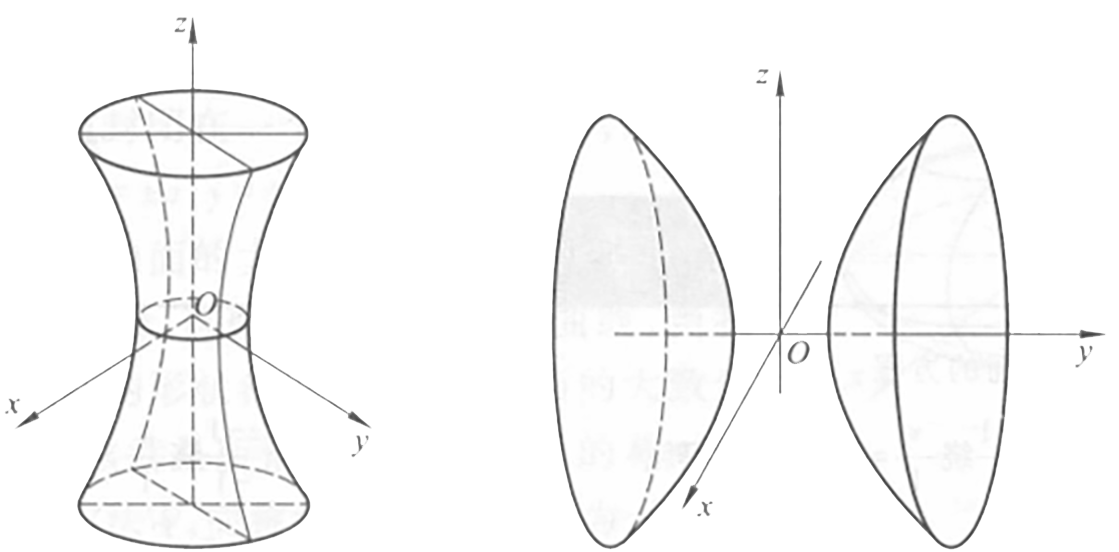
\includegraphics[width=0.6\textwidth]{img/hyperbola.png}
    \caption{Hyperboloids.}
    \label{fig:Hyperboloids}
\end{figure}

\noindent Rotate parabola
\[
\Gamma: \begin{cases} y^{2} = 2pz \\ x = 0, \end{cases}
\]
around \(z\)-axis (axis of symmetry): \(x^{2} + y^{2} = 2pz\) (paraboloid)
(see~\ref{fig:paraboloid}).
\begin{figure}[h]
    \centering
    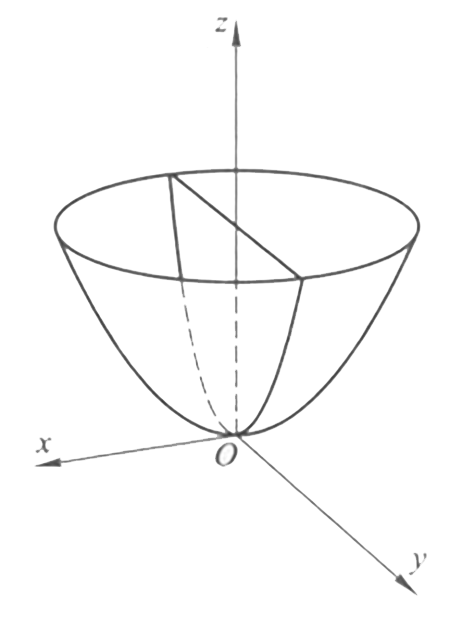
\includegraphics[width=0.2\textwidth]{img/parabola.png}
    \caption{Paraboloid.}
    \label{fig:paraboloid}
\end{figure}

\noindent Rotate circle
\[
\Gamma: \begin{cases} (y-b)^{2}+z^{2}=a^{2}\quad (b>a>0), \\ x = 0, \end{cases}
\]
around \(z\)-axis: \((x^{2}+y^{2}+z^{2}+b^{2}-a^{2})^{2}=4b^{2}(x^{2}+y^{2})\) (torus)
(see~\ref{fig:torus}).
\begin{figure}[h]
    \centering
    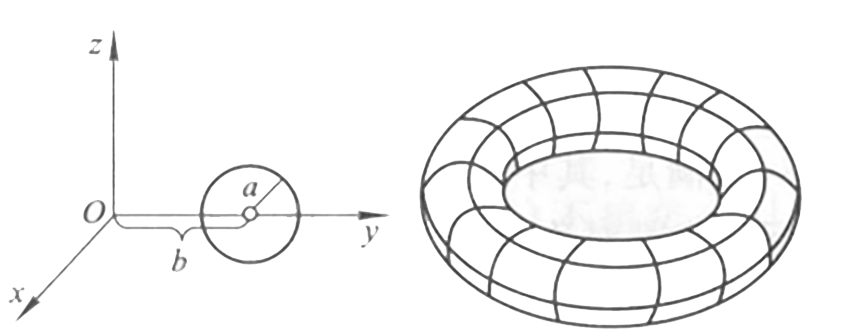
\includegraphics[width=0.5\textwidth]{img/circle.png}
    \caption{Torus.}
    \label{fig:torus}
\end{figure}



\section{Quadric Surfaces}
\begin{leftbarTitle}{Ellipsoids}\end{leftbarTitle}
In space rectangular Cartesian coordinates, 
the surface represented by the equation   
\[ 
\frac{x^{2}}{a^{2}} + \frac{y^{2}}{b^{2}} + \frac{z^{2}}{c^{2}} = 1\quad  (  a  ,  b  ,  c  >  0  )  
\] 
is called an ellipsoid or an ellipsoidal surface, 
and the equation is called the standard equation. 

The parametric equations of the ellipsoid are: 
\[
\begin{cases}
x = a \cos \theta \cos \psi \\
y = b \cos \theta \sin \psi \\
z = c \sin \theta
\end{cases}
\quad   -\frac{\pi}{2} \leq \theta \leq \frac{\pi}{2},\quad 0 \leq \psi \leq 2\pi.
\]

Any ellipsoid with two equal axes is necessarily a spheroid, 
and an ellipsoid with three equal axes is a sphere. 

The surface can be studied by \textbf{the method of parallel sections}, i.e., 
by using the cross-sections of parallel planes to study the shape of the surface. 

Use a set of parallel planes \(z=h\) to section the ellipsoid~(\ref{fig:Ellipsoid1}), i.e., 
\[
\{ (x,y,z) | F(x,y,z) = 0 \} = 
\bigcup_{-h \leq z \leq h} \{ (x,y) | \frac{x^{2}}{a^{2}} + \frac{y^{2}}{b^{2}} = 1 - \frac{h^{2}}{c^{2}}\}.
\]      
Obviously, when \(|h| = c\) , the section is a point; 
when \(|h| < c\) , the section is an ellipse. 
The other two methods of sectioning are similar.
\begin{figure}[h]
    \centering
    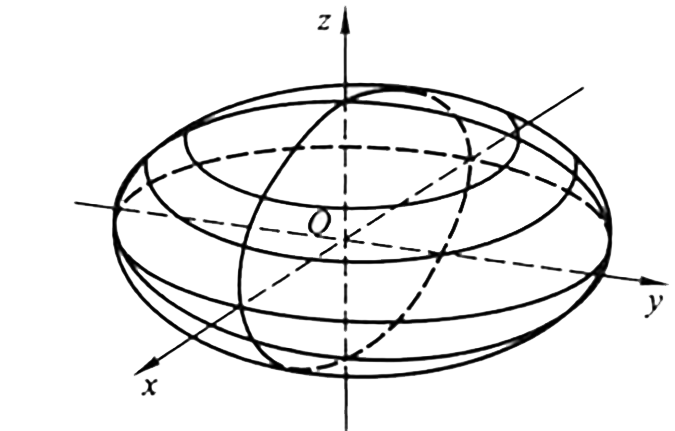
\includegraphics[width=0.5\textwidth]{img/Ellipsoid.png}
    \caption{Ellipsoid.}
    \label{fig:Ellipsoid1}
\end{figure}

\begin{leftbarTitle}{Hyperboloids}\end{leftbarTitle}
In space rectangular Cartesian coordinates, 
the surface represented by the equation
\[
\frac{x^{2}}{a^{2}} + \frac{y^{2}}{b^{2}} - \frac{z^{2}}{c^{2}} = 1\quad (a,b,c > 0)
\]
is called a one-sheet hyperboloid.

\begin{enumerate}[label=\roman*.]
    \item Use a set of parallel planes \(z=h\) to section the one-sheet hyperboloid~(\ref{fig:OneSheetHyperboloid}), i.e.,
        \[
        \{ (x,y,z) | F(x,y,z) = 0 \} = 
        \bigcup_{-\infty < z < \infty} \{ (x,y) | \frac{x^{2}}{a^{2}} + \frac{y^{2}}{b^{2}} = 1 + \frac{h^{2}}{c^{2}}\}.
        \]
        The section is always an ellipse.
        \begin{figure}[h]
            \centering
            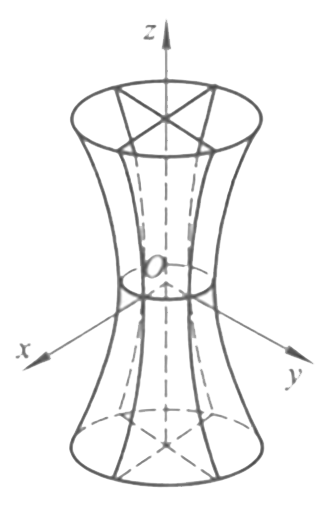
\includegraphics[width=0.2\textwidth]{img/one-sheet-hyperboloid1.png}
            \caption{One-sheet hyperboloid.}
            \label{fig:OneSheetHyperboloid}
        \end{figure}
    \item Use a set of parallel planes \(y=h\) to section the one-sheet hyperboloid~(\ref{fig:OneSheetHyperboloid2}), 
        the section is
        \[
        \begin{cases} \frac{x^{2}}{a^{2}} + \frac{z^{2}}{c^{2}} = 1 - \frac{h^{2}}{b^{2}}, \\ y=h.  \end{cases}
        \]
        When \(|h| < b\), the section is a hyperbola;\newline
        when \(|h| = b\), the section is two parallel lines, i.e., 
        \[
        \begin{cases} \frac{x}{a}\pm \frac{z}{c} = 0, \\ y=b ,\end{cases}
        \text{or}
        \begin{cases} \frac{x}{a}\pm \frac{z}{c} = 0, \\ y=-b ;\end{cases}
        \]
        when \(|h| > b\), the section is a hyperbola.
        \begin{figure}[h]
            \centering
            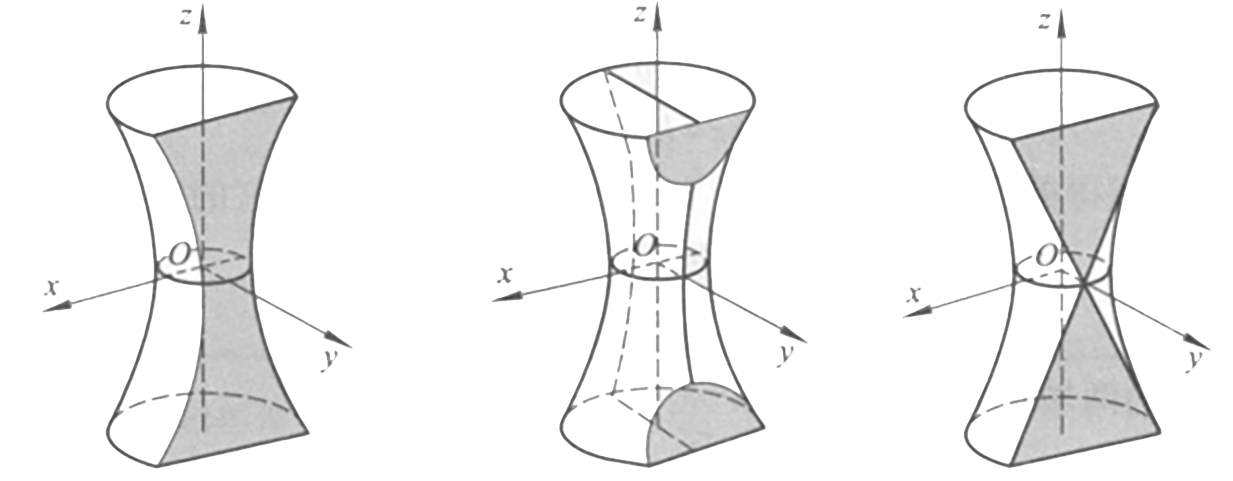
\includegraphics[width=0.5\textwidth]{img/one-sheet-hyperboloid2.png}
            \caption{One-sheet hyperboloid.}
            \label{fig:OneSheetHyperboloid2}
        \end{figure}
\end{enumerate}

In space rectangular Cartesian coordinates, 
the surface represented by the equation
\[
\frac{x^{2}}{a^{2}} + \frac{y^{2}}{b^{2}} - \frac{z^{2}}{c^{2}} = -1\quad (a,b,c > 0)
\]
is called a two-sheet hyperboloid.

\vspace{0.7cm}
Use a set of parallel planes \(z=h\) (\(|h|\geqslant c\)) to section the two-sheet hyperboloid~(\ref{fig:TwoSheetHyperboloid}), 
the section is
\[
\begin{cases} \frac{x^{2}}{a^{2}} + \frac{y^{2}}{b^{2}} = 1 + \frac{h^{2}}{c^{2}}, \\ z=h. \end{cases}
\]
When \(|h| > c\), the section is an ellipse;\newline
when \(|h| = c\), the section is a point.
\begin{figure}[h]
    \centering
    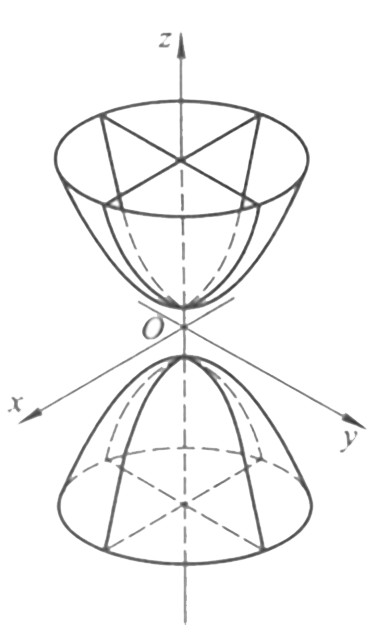
\includegraphics[width=0.2\textwidth]{img/two-sheet-hyperbloid.png}
    \caption{Two-sheet hyperboloid.}
    \label{fig:TwoSheetHyperboloid}
\end{figure}

\begin{leftbarTitle}{Paraboloids}\end{leftbarTitle}
In space rectangular Cartesian coordinates, 
the surface represented by the equation
\[
\frac{x^{2}}{a^{2}} + \frac{y^{2}}{b^{2}} = 2z\quad (a,b > 0)
\]
is called an elliptic paraboloid.
\begin{enumerate}[label=\roman*.]
    \item Use a set of parallel planes \(z=h\) (\(h\geqslant 0\)) to section the elliptic paraboloid.
        When \(h>0\), the section is an ellipse;\newline
        when \(h=0\), the section is a point.
    \item Use a set of parallel planes \(y=h\) to section the elliptic paraboloid~(\ref{fig:EllipticParaboloid}),
        the section is a parabola, whose equation is
        \[
        \begin{cases} x^{2} = 2a^{2}(z-\frac{h}{2b^{2}}), \\ y=h. \end{cases}
        \]
        \begin{figure}[h]
            \centering
            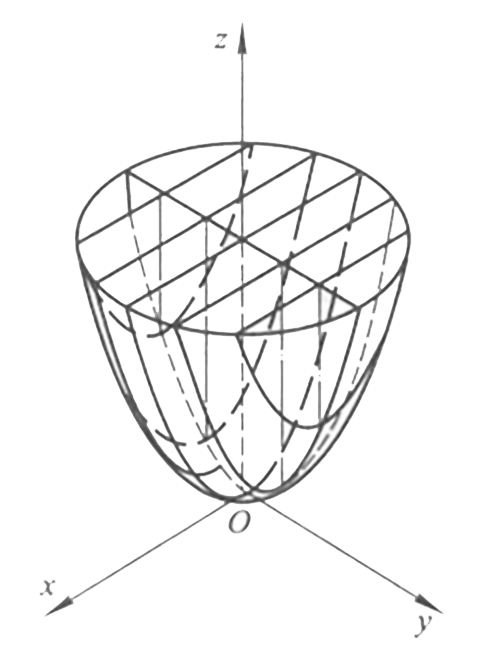
\includegraphics[width=0.3\textwidth]{img/elliptic-paraboloid.png}
            \caption{Elliptic paraboloid.}
            \label{fig:EllipticParaboloid}
        \end{figure}
\end{enumerate}

\vspace{0.7cm}
In space rectangular Cartesian coordinates, 
the surface represented by the equation
\[
\frac{x^{2}}{a^{2}} - \frac{y^{2}}{b^{2}} = 2z\quad (a,b > 0)
\]
is called a hyperbolic paraboloid, or a saddle surface.
\begin{enumerate}
    \item Use a set of parallel planes \(z=h\) to section the hyperbolic paraboloid~(\ref{fig:HyperbolicParaboloid1}).
        When \(h\neq 0\), the section is a hyperbola
        \[
        \begin{cases} \frac{x^{2}}{2a^{2}h} - \frac{y^{2}}{2b^{2}h} = 1, \\ z=h; \end{cases}
        \]
        and if \(h>0\), the real axis of hyperbola is parallel to the \(x\)-axis;
        if \(h<0\), the real axis of hyperbola is parallel to the \(y\)-axis;\newline
        when \(h=0\), the section is two lines intersecting at the origin, i.e.,
        \[
        \begin{cases} \frac{x}{a}\pm \frac{y}{b} = 0, \\ z=0. \end{cases}
        \]
        \begin{figure}[h]
            \centering
            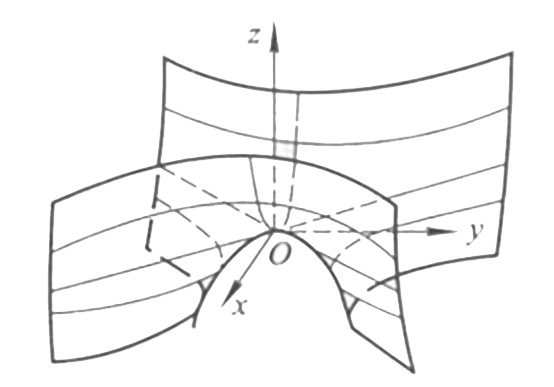
\includegraphics[width=0.3\textwidth]{img/hyperbolic-paraboloid1.png}
            \caption{Hyperbolic paraboloid.}
            \label{fig:HyperbolicParaboloid1}
        \end{figure} 
    \item Use a set of parallel planes \(y=h\) to section the hyperbolic paraboloid~(\ref{fig:HyperbolicParaboloid2}),
        the section is a parabola, whose equation is
        \[
        \begin{cases} x^{2} = 2a^{2}(z+\frac{h}{2b^{2}}), \\ y=h. \end{cases}
        \]
        \begin{figure}[h]
            \centering
            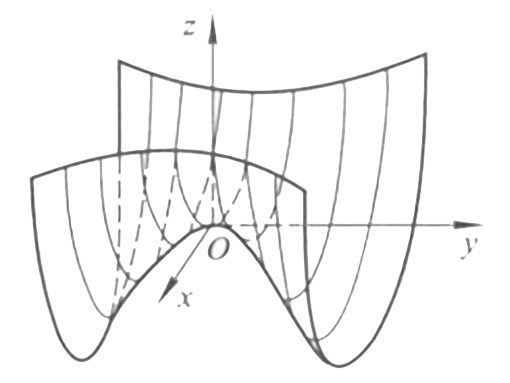
\includegraphics[width=0.3\textwidth]{img/hyperbolic-paraboloid2.png}
            \caption{Hyperbolic paraboloid section.}
            \label{fig:HyperbolicParaboloid2}
        \end{figure}
\end{enumerate}

\section{Ruled Surfaces}
\begin{definition}{Ruled Surface}
    In space, the surface generated by a family of straight lines is called a \textbf{ruled surface},
    such a family of straight lines is called a family of \textbf{straight generatrices} of the surface.
\end{definition}

\begin{proposition}
    \begin{enumerate}
        \item One-sheet hyperboloid and hyperbolic paraboloid are ruled surfaces. 
        \item For any point on a one-sheet hyperboloid or hyperbolic paraboloid, 
            there is exactly one straight line from each of the two families of straight generatrices 
            that passes through the point.
        \item Any two straight generatrices from different families on a hyperboloid of one sheet must be coplanar, 
            while any two straight generatrices from different families on a hyperbolic paraboloid must intersect.
        \item Any two straight generatrices of the same family on a one-sheet hyperboloid or a hyperbolic paraboloid 
            are always skew lines, 
            and all straight generatrices of the same family on a hyperbolic paraboloid are parallel to the same plane.
    \end{enumerate}
\end{proposition}

\begin{figure}[h]
    \centering
    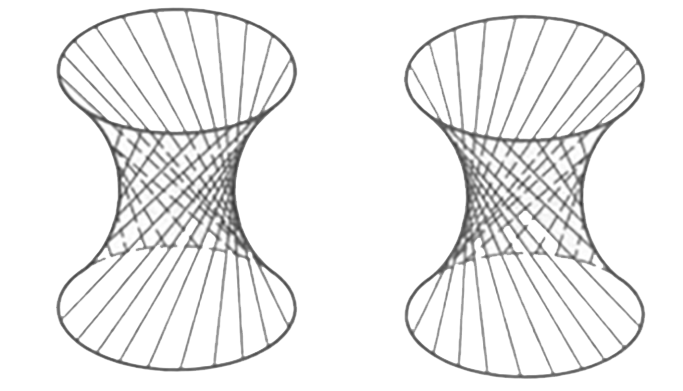
\includegraphics[width=0.5\textwidth]{img/ruled-surface1.png}
    \caption{One-sheet hyperboloid.}
    \label{fig:RuledSurface1}
\end{figure}

\begin{figure}[h]
    \centering
    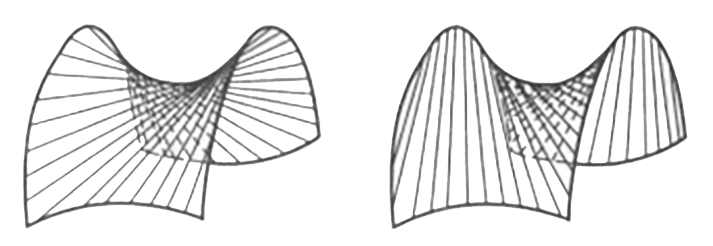
\includegraphics[width=0.5\textwidth]{img/ruled-surface2.png}
    \caption{Hyperbolic paraboloid.}
    \label{fig:RuledSurface2}
\end{figure}


\chapter{Conic Sections}
\section{General Equation of Conic Sections}

\begin{figure}[h]
    \centering
    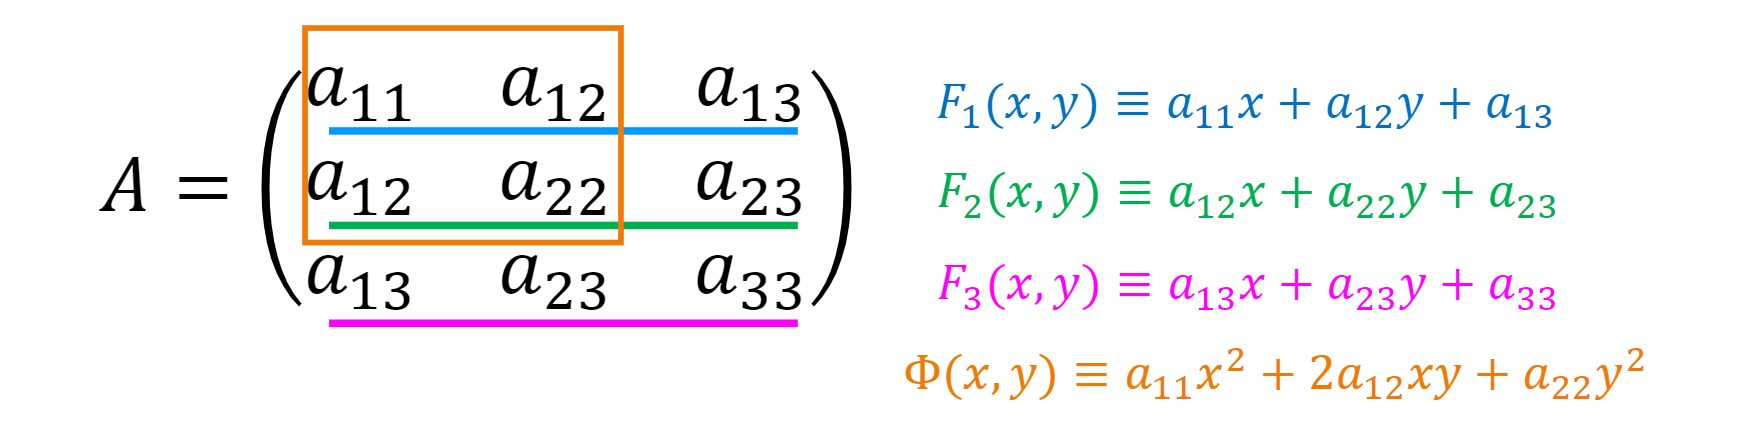
\includegraphics[width=0.8\textwidth]{img/ConicRelation.png}
\end{figure}

\section{Conic Sections and Lines}

\section{Simplification of Conic Equations}

\chapter{Quadric Surfaces}



\begin{thebibliography}{99} 
\bibitem{en1} 作者, Title1, Journal1, Year1. \emph{ This is an example of a reference.}
\bibitem{en2} Author2, Title2, Journal2, Year2. \emph{ This is another example of a reference.}
\end{thebibliography}

\end{document}